\chapter{Experiments}\label{experiments}
As shown in figure~\ref{fig:process}, the main experimental setup can be structured into four parts.
In a preprocessing step, we standardize the Gutenberg dataset to the new PAN 2020 format and we clean the Fanfiction dataset.
Then, we transcribe the datasets using the phonetic transcription methods defined earlier.
The resulting datasets, as well as the original dataset, are then used as the inputs to two widely used Authorship Verification algorithms which are described in more detail in this chapter.
For all experiments, we conduct three cross-validation runs with ten folds each.
We then average the results and compute the Bonferroni-corrected\footnote{As we conduct 30 runs on the same data, the likelihood of encountering a rare configuration that performs well and accepting it as statistically significant is high. Thus we divide the $p$-values for accepting statistical significance by 30.} statistical significance using a paired t-test as the test statistic.
Finally, we analyze the results.
\begin{figure}
  \centering
  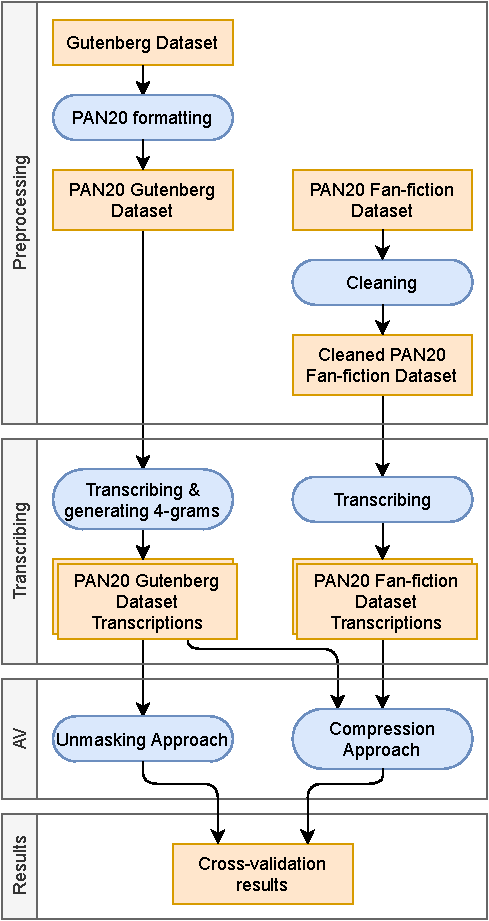
\includegraphics[width=0.6\textwidth]{figures/process}
  \caption{Experimental setup, orange = data, blue = process.}
  \label{fig:process}
\end{figure}

% 1.2 Compression Approach
\section{Compression Approach}\label{sec:compression-approach}
The first approach, originally from \cite{teahan2003compression} and later adapted to Authorship Verification and employed as a benchmark in PAN 2020, uses a text compression method to determine the chance that two texts were written by the same author.
Text compression can be seen as encoding a given text with an encoding that is optimized for this text.
As discussed in \cite{brown1992upperBoundEntropy}, by determining this encoding, text compression can be used to estimate an upper bound to the entropy, i.e., the amount of information of characters in English text.
More specifically, by using the compression model optimized on some text A, the cross-entropy of encoding a text B with this model can be calculated.
During training, this is done for each pair in both directions.
The mean and average of the distance between the resulting cross-entropies are then used to train a logistic regression model.
The smaller the resulting difference, the more similar the texts, and the higher the chance that both are written by the same author.
The compression model used is Prediction by Partial Matching (PPM), a standard algorithm for lossless text compression, first introduced by \cite{cleary1984PPM}.
As done in PAN 2020, we employ an uncertainty interval with a radius of 5\%, i.e., predictions that are in the interval $[0.45,~0.55]$ are given a \textit{non-answer} classification.
The source code used is based on a reimplementation of the Authorship Attribution approach from \cite{teahan2003compression} as part of a reproducibility study in \cite{potthast2016reimplementation}.
The adaption for Authorship Verification stems from PAN 2020\footnote{\url{https://github.com/pan-webis-de/pan-code/tree/master/clef20/authorship-verification}}.
The source code extending the algorithm to use phonetic features and adding cross-validation functionality is available on GitHub\footnote{\url{https://github.com/av-pt/teahan03-phonetic}}.
% Add figure, only showing cross-validation side!

% 1.3 Unmasking Approach
\section{Unmasking Approach}\label{sec:unmasking-approach}
Unmasking was first introduced by \citeauthor{koppel2004unmasking} in 2004.
In short, it exploits the degradation of classifier accuracy when removing distinguishing features.
It turns out that iteratively removing those features leads to a faster degradation on text pairs by one author than on those by different authors.
Thus, the algorithm ``unmasks'' the text pairs and thereby reveals the information needed for classification.\\
% Formal definiton & explanation: unmasking step
This approach comprises two steps: First, a cross-validation method is employed to create the accuracy degradation curves for all training samples.
Second, a meta-classifier is trained on the resulting curves to differentiate between same-author and different-author curves.\\
%XXX From here on!
%For a given pair, the texts are seen to be created by two generative processes $p_1$ and $p_2$.
To compute a curve for a pair, both texts are chunked into parts longer than 500 words without splitting paragraphs.
The 250 words with highest average frequencies in the two texts are used as features.
In a 10-fold cross-validation, linear support vector machine (SVM) models are trained to classify if a chunk belongs to the first or the second text.
The resulting accuracy is noted and the three most discriminating positive and negative features are removed from the feature set.
The cross-validation and feature removal are repeated until no features are left.\\
% meta-learning step
The set of curves is then used to train a linear SVM model as a meta-classifier.
As brought to the point by \cite{bevendorff2019unmaskingShortTexts}, the features used are ``the curve points, the curves' point-wise first- and second-order derivatives, and the derivatives sorted by steepest point-wise drop''.\\
% Adaptation for short texts by Bevendorff et al., how is this different? Which features are actually being used?
Unmasking is one of the most robust Authorship Verification algorithms.
But as it requires sufficient chunks of no less than 500 words in length, it is only applicable for book-length texts.
To counter this, \cite{bevendorff2019unmaskingShortTexts} generalizes the algorithm to accommodate for short texts.
Chunks are generated by oversampling the bag-of-words pool of a given text.
Words from this pool are picked randomly without replacement until a length of 700 words is reached and the pool is reset afterwards.
In total, 30 chunks are generated which are then used for curve generation as above with the only exception that the five most positive and negative features are removed instead of only three.
As this approach introduces a significant amount of variance in the resulting curves, the Unmasking step is repeated multiple times and the curves are averaged.
It is recommended to average at least 15--20 Unmasking runs for each text pair.
In our experiments, we average the curves of 32 Unmasking runs per text pair with varying chunk sizes of 500, 600, and 700 words respectively.
In the implementation supplied by \cite{bevendorff2019unmaskingShortTexts}\footnote{\url{https://github.com/webis-de/unmasking}} and used as the basis for our research, the meta-classifier uses the curves' ``central-difference gradients (first- and second-order), as well as their gradients sorted by magnitude''.
Also, the implementation predicts labels instead of confidence values, hence reducing $F_{0.5u}$ to $F_{0.5}$\footnote{Weighting precision two times as much as recall, but not accounting for \textit{non-answers}.} and $c@1$ to accuracy.
The source code extending the Unmasking framework for the use of phonetically transcribed datasets and implementing a cross-validation functionality is available on GitHub\footnote{\url{https://github.com/av-pt/unmasking}}.
Note that we only use the Gutenberg dataset for Unmasking as processing the larger Fanfiction dataset for each transcription proved to be too time-consuming.